\section{Background and Motivation}
\label{hpca:sec:background}

Branch prediction unit predicts the program control flow and supplies a stream of instruction addresses/program counters (PCs) on the predicted path to the fetch unit which fetches the corresponding instructions to feed the rest of the core. As branch instructions disturb the otherwise sequential control flow, the branch prediction unit needs to identify them to predict the upcoming control flow. However, whether an instruction is a branch or not can only be determined after it has been fetched and decoded. To avoid the latency of fetching and decoding instructions before generating next PCs, the branch prediction unit employs a special hardware structure, called branch target buffer (BTB), to identify branch instructions solely from their PCs before the instructions themselves are even fetched.

\subsection{Branch Target Buffer (BTB)}
%\runinsec{Branch Target Buffer (BTB)}
%BTB is used in the branch prediction unit to identify whether a PC corresponds to a branch instruction before the instruction itself is even fetched.
\Cref{hpca:fig:conv-btb} presents the conventional BTB organization. Each BTB entry consists of \textit{valid}, \textit{tag}, \textit{type}, \textit{target}, and \textit{rep\_policy} fields. \Cref{hpca:fig:conv-btb} also shows the typical number of bits needed for these fields. The \textit{tag} field usually stores only a partial tag, which is generated by hashing the full tag, to reduce storage cost while introducing minimal aliasing. The number of bits for \textit{target} field depends on the size of virtual address space and instruction set architecture (ISA). We assume a 48-bit virtual address space and ARMv8 ISA to calculate target field size in \Cref{hpca:fig:conv-btb}. As ARMv8 instructions are always 32-bits and 4-byte aligned, the least significant two bits of a PC are always zeros. Therefore, we only need 46-bits for the \textit{target} field. The \textit{valid} bit indicates whether the entry contains valid information or not, while \textit{rep\_policy} bits choose one of the existing branches for eviction when a new branch is inserted in the BTB.

To check whether a PC corresponds to a branch instruction, the BTB is indexed, i.e. accessed, with the low order PC bits. The high order PC bits are hashed, using the same function that is used to generate partial tags, and compared to the \textit{tag} field of the indexed BTB entry. A match indicates that the PC belongs to a branch. 

A branch instruction simply implies the presence of a potential control flow divergence point in program execution. However, whether or not the divergence actually happens depends on the type of branch, i.e. call, return, conditional, or unconditional branch, which is stored in the \textit{type} field of a BTB entry. Call, return, and unconditional branches always cause control flow divergence as they are always \textit{taken}. Conditional branches, in contrast, are not always taken and a direction predictor is used to predict their direction. 

If a branch is predicted to be taken, the \textit{target} field in the BTB entry provides the address for the next instruction, except for returns. This is because the return address is call-site dependent and a given function can be called from different call sites. Therefore, a return address stack (RAS) is typically employed to record return addresses at call-sites. On a function call, the call instruction pushes the return address to RAS, which is later popped by the corresponding return instruction.

\subsection{The cost of a BTB miss}
%\runinsec{The cost of a BTB miss}
A BTB miss for a branch instruction means that the branch is undetected and the front-end continues to fetch instructions sequentially. Whether or not the sequential path is the correct one depends on the actual direction of the missed branch. Unless the missed branch is a conditional branch that is not taken, the sequential path is incorrect. When the wrong path is eventually detected by the core, all the instructions after the branch that missed in the BTB are flushed, fetch is redirected to the branch target and pipeline is filled with correct-path instructions. BTB misses are thus highly deleterious to performance as they result in a loss of tens of cycles of work and expose the pipeline fill latency. 

\begin{figure}
\centering
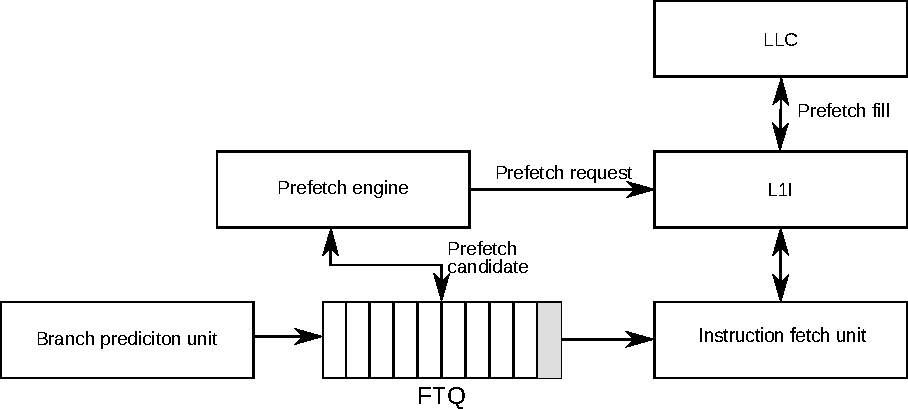
\includegraphics[width=.9\columnwidth, trim=0 0 0 0, clip]{figures/fdip1.pdf}
\caption{FDIP microarchitecture}
\label{hpca:fig:fdip}
\end{figure}


\subsection{BTB's role in instruction prefetching}
%\runinsec{BTB's role in instruction prefetching}
Fetch-directed instruction prefetchers are a class of powerful L1-I prefetchers that intrinsically rely on BTB to identify prefetch candidates. 
These prefetchers are highly effective and, when coupled with a sufficiently large BTB, outperform the winner of the recently-concluded Instruction Prefetching Championship~\cite{ipc1} and approach the performance of an ideal L1-I, as reported by Ishii et al.~\cite{rebase}. Variants of these prefetchers have been adopted in commercial products, for example in IBM z15~\cite{IBMz15HotChips}, ARM Neoverse N1~\cite{neoverse} etc.

\Cref{hpca:fig:fdip} shows a canonical organization of a fetch-directed instruction prefetcher (FDIP)~\cite{fdip}. 
As originally proposed, FDIP decouples the branch-prediction unit and the fetch engine via the {\em fetch target queue (FTQ)}. This decoupling allows the branch prediction unit to run ahead of the fetch engine and discover prefetch candidates by predicting the control flow far into the future. With FDIP, each cycle, the branch prediction unit identifies and predicts branches to anticipate upcoming execution path and inserts corresponding instruction addresses into the FTQ. Consequently, the FTQ contains a stream of anticipated instruction addresses to be fetched by the core. The prefetch engine scans the FTQ to identify prefetch candidates and issue prefetch requests. 

For FDIP to be effective, the BTB needs to accommodate the branch working set, otherwise frequent BTB misses will cause FDIP to prefetch the wrong path as FTQ will be filled with wrong path instruction addresses. This is one of the key reasons why commercial processors deploy massive BTBs, as also observed by~\cite{rebase}. These massive BTBs incur astronomical storage overheads. Also, not only the BTB storage overhead is high, it is increasing at a rapid pace. For example, \Cref{hpca:tab:btbcap}, presents the BTB storage cost in several generations of Samsung Exynos processors. As the table shows, the BTB storage cost nearly doubled in each generation, except between M4 and M5. Overall, the storage cost increased nearly six fold (98.9KB to 561.5KB) from M1 to M6, over a period of about eight years~\cite{exynos}.

As the instruction footprints of server applications continue to expand, a trend also reflected in Google Web Search workload whose instruction footprint is growing at annualized rate of 27\%~\cite{profileWarehouse}, the BTB sizes and their storage overheads are destined to increase in future. Therefore, there is an urgent need to investigate storage-effective BTB organizations to combat the front-end bottleneck without necessitating prohibitive area budgets.

\begin{table}[t]
  \centering
  \caption{\label{hpca:tab:btbcap} BTB storage cost in Samsung Exynos processors}
  \begin{tabular}{ll}\hline
    \textbf{CPU} & \textbf{BTB Storage} \\\hline
    M1/M2 & 98.9KB \\
    M3 & 175.8KB \\
    M4 & 288.0KB \\
    M5 & 310.8KB \\
    M6 & 561.5KB \\\hline
  \end{tabular}
\end{table}

%To avoid the storage and area overhead of large BTBs, the academic community is investigating alternate mechanisms to improve FDIP while employing reasonably sized BTBs. For example, Boomerang~\cite{boomerang} avoids wrong path prefetching under BTB misses. To do so, it detects BTB misses, by using BBTB, and fills the missed BTB entries, by fetching and pre-decoding the appropriate cache blocks, before predicting the upcoming control flow and populating FTQ entries. Shotgun~\cite{shotgun} proposed a new BTB organization to maximize the control flow captured in a limited size BTB, thus reducing BTB misses and their negative impact on prefetching.

%\begin{table}
%  \centering
%  \caption{\label{hpca:tab:btbcap} BTB capacity of commercial CPUs}
%  \begin{tabular}{ll}\hline
%    \textbf{CPU} & \textbf{Capacity} \\\hline
%    IBM z-series processors~\cite{IBMz} & 24K \\
%    AMD Zen-2~\cite{zen2} & 8.5K \\
%    ARM Neoverse N1~\cite{neoverse} & 6K \\
%    Samsung Exynos M3~\cite{rupley2018samsung} & 16K \\\hline
%  \end{tabular}
%\end{table}



